\documentclass[10pt,a4paper]{article}
\usepackage[margin=2.2cm]{geometry}
\usepackage{fontspec}
\usepackage{kotex}
\setmainfont{Apple SD Gothic Neo}
\setsansfont{Apple SD Gothic Neo}
\usepackage{amsmath,amssymb}
\usepackage{graphicx}
\usepackage{booktabs}
\usepackage{caption}
\usepackage[dvipsnames]{xcolor}
\usepackage[colorlinks=true,linkcolor=MidnightBlue,citecolor=MidnightBlue,
            urlcolor=MidnightBlue]{hyperref}
\usepackage{titlesec}
\titleformat{\section}{\large\bfseries}{\thesection}{0.6em}{}
\titleformat{\subsection}{\normalsize\bfseries}{\thesubsection}{0.5em}{}
\captionsetup{font=small,labelfont=bf}
\setlength{\parskip}{0.35em}
\setlength{\parindent}{0pt}

\usepackage{mdframed}
\newmdenv[linewidth=0.4pt,linecolor=gray!60,backgroundcolor=gray!5,
          innertopmargin=6pt,innerbottommargin=6pt,skipabove=8pt,skipbelow=8pt]{claimbox}
\newcommand{\claim}[2]{\begin{claimbox}\textbf{주장.} #1\par\smallskip
  \textcolor{gray!70}{\textbf{반증 조건.} #2}\end{claimbox}}

\title{\bfseries 겹친 만큼 잃는다\\[2pt]
\large 판 0 은 무신호가 아니라 상쇄였다}
\author{월드모델 실험실 · 노트 675}
\date{2026-08-06}
\begin{document}\maketitle

\section{한 줄}

새 축을 판에 붙였더니 신호 몫이 $-0.0004$ --- 사실상 0 이다. 여기서 멈추면
``정보가 없다''로 끝난다. 도메인별로 갈라 보니 \textbf{양수 둘과 음수 셋이
상쇄}한 것이고, 어느 쪽이 될지는 \textbf{기존 축과의 겹침}이 정한다 ---
스피어만 $\mathbf{-1.000}$. 그리고 \textbf{위약에는 그 무늬가 없다.}

\section{왜 이걸 했나}

노트 668 과 674 가 지역 방문자 축의 두 확장 경로를 다 닫았다. 남은 물음이
\emph{``장소가 없는 도메인에서 (시간 $\times$ 대상) 을 만드는 것이 무엇인가''}였고,
후보가 하나 있었다 --- 노트 670 이 결함을 고친 \verb|crowd_share|(직전 90일
\textbf{갈래별} 출시 몫의 평균).

이 축이 매력적인 이유는 \textbf{두께}다. 방문자 축은 두 도메인에만 붙어 유보 가중
$0.057$ 인데 이 축은 다섯 도메인에 붙어 \textbf{$0.530$} 이다 --- \textbf{9.3배}.
판 문턱 $0.0045$ 를 넘으려면 다섯 도메인이 고르게 오를 때 \textbf{각
$+0.0085$} 면 되고, 방문자 축은 각 $+0.079$ 가 필요했다(실제로 팝업이 $+0.009$
였으니 11\%만 왔다). \textbf{그 계산을 결과 전에 적었다.}

\section{쟀다 --- 세 팔}

\begin{center}
\begin{tabular}{lrrr}
\toprule
팔 & 판 & 차 & 양수 \\
\midrule
① 없이 & 0.4689 & --- & --- \\
② 진짜 & 0.4671 & $-0.0018$ & 2/12 \\
③ 위약 & 0.4675 & $-0.0014$ & 0/12 \\
\bottomrule
\end{tabular}
\end{center}

\textbf{신호 몫 $= -0.0004$.} 문턱은 $0.0045$ 다. 노트 335 의 판정 조건이 그대로
성립한다 --- \emph{위약이 진짜보다 나쁘지 않으면 신호가 아니라 차원 비용이다.}
사전등록 규칙 ③ 이 발동해서 \textbf{판 수준에서 축을 닫는다.}

내 예측은 ``신호 몫만 문턱을 넘는다($+0.0045\sim0.008$)''였고 \textbf{틀렸다.} 근거로
적은 셋 중 둘(축$\leftrightarrow$라벨 $|r|$ $0.105$ · 덮음 세 배)은 사실이지만 판
효과로 이어지지 않았다. 맞았던 것은 셋째 --- \emph{``창 불변 · 자기상관 $0.85$ 는
느리게 변하는 수준이라는 뜻이고, 수준 축은 노트 649 가 실패시킨 모양에 가깝다.''}
\textbf{그 경고를 예측의 근거로 쓰고 예측의 반대편으로는 안 썼다.}

\section{그런데 0 의 정체가 다르다}

관문 ③(기존 축과의 상관 · 노트 651)을 재면 다섯 도메인 \emph{전부} 최대 상관이
\verb|gen| 이고 값이 갈린다: 만화 $0.316$ · 세계애니 $0.403$ · 게임 $0.573$ ·
애니 $0.683$ · 모바일 $0.770$. 그 순서로 도메인 신호 몫을 늘어놓으면 이렇게 된다.

\begin{figure}[t]\centering
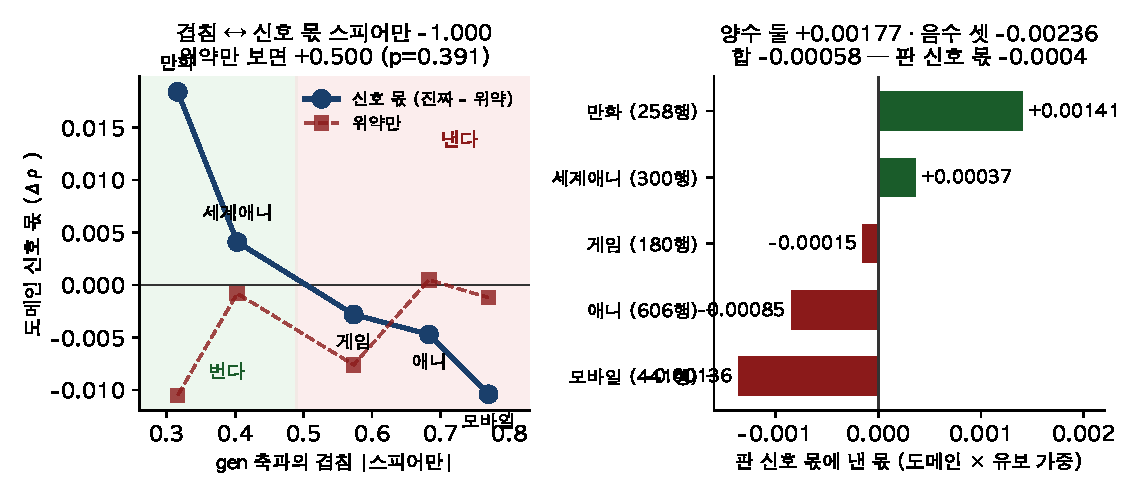
\includegraphics[width=0.99\textwidth]{figs/dose.pdf}
\caption{왼쪽: 겹침이 커질수록 신호 몫이 단조 감소하고 $\approx 0.5$ 에서 부호가
바뀐다(스피어만 $-1.000$ · 피어슨 $-0.942$ · $n{=}5$). \textbf{위약만 보면
$+0.500$($p{=}0.391$)로 무늬가 없다} --- 기울기는 ``어느 도메인이 열 하나에
약한가''가 아니라 축의 정보 내용에서 온다. 오른쪽: 유보 가중을 곱하면 양수 둘이
$+0.00193$, 음수 셋이 $-0.00251$ 로 상쇄해서 합이 $-0.00058$ 이다.}
\end{figure}

\claim{\textbf{관문 ③ 은 거부권이 아니라 용량 함수다.} 노트 651 이 그것을
``$|r| \ge 0.85$ 면 무효''라는 문턱으로 세웠는데, 실제로는 문턱 아래 전 구간에서
\textbf{겹침이 얼마면 얼마를 잃는지}가 정해진다. 겹침 $0.32$ 에서 $+0.0184$,
$0.77$ 에서 $-0.0104$ 다.}
{$n{=}5$ 이고 $p{=}0.037$ 이라 한 도메인이 뒤집히면 스피어만이 무너진다. 그리고
겹침이 갈래 어휘의 풍부함과 상관될 수 있다 --- 그 교란은 안 쟀다. 다른 축에서
같은 기울기가 재현되지 않으면 이 주장은 이 축의 특성이다.}

\claim{\textbf{판 신호 몫 0 을 ``정보 없음''으로 읽으면 안 된다.} 여기서 0 은
\textbf{상쇄}다. 겹침이 낮은 두 도메인에서 축은 실제로 정보를 넣는다 --- 만화
$+0.0184$ 는 그 도메인 혼자 판 문턱을 넘는 데 필요한 $+0.0588$ 의 \textbf{31\%}다.}
{도메인별 차가 이웃 효과라면 이 읽기가 무너진다. 이 팔에서 축이 안 붙은 여섯
도메인의 몫 합은 $\mathbf{+0.00013}$ 으로 사실상 0 이라 \emph{전역 팔에서는} 이웃
효과가 없다. \textbf{그러나 단일 전환에서의 이웃 효과는 다른 물음이고 안 쟀다.}}

\section{여기서 처방을 만들지 않는다}

겹침이 낮은 둘(만화 · 세계애니)에만 축을 붙이면 될 것 같다. \textbf{그렇게 하지
않는다.} 노트 551 · 560 · 563 이 \textbf{세 번} 쟀다 --- \emph{전역 변경의 도메인별
차로 후보를 세우면 그 도메인만 바꿀 때 부호가 뒤집힌다}(도서 $+0.0459 \to
\mathbf{-0.0820}$ · 게임 $-0.0137 \to \mathbf{+0.0138}$).

다만 이번은 앞선 셋과 다른 점이 하나 있다. 그때는 도메인을 \textbf{결과를 보고}
골랐고, 이번에는 \textbf{사전 예측자}가 있다 --- 겹침은 라벨을 안 보고 계산된다.
그래서 다음 실험은 \emph{고르기}가 아니라 \emph{예측}이다: 단일 전환으로 만화 ·
세계애니만 붙이고, \textbf{전역 표가 예측한 부호가 유지되나}를 본다. 판정 둘을
따로 적었다 --- (가) 부호 유지 여부 (나) 판 문턱 통과 여부. 기대 판 이득은 유보
가중으로 $+0.0018$ 이라 \textbf{(나)는 미달할 것}이고, 그래도 (가)를 재는 이유는
그것이 조항의 시험이기 때문이다.

\section{남는 것}

이 축의 순효과가 음수인 것($-0.0018$)은 차원 비용이고 그 비용은 작다 ---
위약 $-0.0014$ 다(방문자 축 위약은 $-0.0048$). \textbf{다섯 도메인이 두꺼우면
열값이 작다}는 노트 641 의 열 예산이 여기서도 그대로 맞는다. 즉 이 축의 문제는
비용이 아니라 \textbf{정보가 절반은 이미 있는 것}이다.

\end{document}
